\documentclass[]{article}
%Busca la linea que pone /tableofcontents y empieza a escribir debajo de cada sección.
%Te explico para qué es cada cosa que sea medio relevante:
\usepackage{amsmath}
\usepackage{amssymb}
\usepackage{verbatim} %con verbatim escribes bloques de texto con letra mono.
\usepackage{graphicx} %para insertar imagenes, cuando meta yo una usa el codigo de ejemplo
\usepackage{float}
\usepackage{listings}
\usepackage{fullpage}
\usepackage{color}
\usepackage{fancyvrb}
\usepackage[spanish]{babel}
\usepackage[utf8]{inputenc} %Para usar acentos directamente en latex
\usepackage{hyperref} %Para que el indice tenga hiperenlaces y si quieres poner los tuyos
\hypersetup{%
	pdfborder = {0 0 0}
}

\definecolor{mygreen}{rgb}{0,0.6,0}
\definecolor{mygray}{rgb}{0.5,0.5,0.5}
\definecolor{mymauve}{rgb}{0.58,0,0.82}

%Para insertar código: crea un recuadro con texto mono y lineas enumeradas. Puedes referenciar un fichero y no copiar y pegar aquí.
\lstset{ %
	backgroundcolor=\color{white},   % choose the background color; you must add \usepackage{color} or \usepackage{xcolor}
	basicstyle=\footnotesize,        % the size of the fonts that are used for the code
	breakatwhitespace=false,         % sets if automatic breaks should only happen at whitespace
	breaklines=true,                 % sets automatic line breaking
	captionpos=b,                    % sets the caption-position to bottom
	commentstyle=\color{mygreen},    % comment style
	 keywordstyle=\color{blue}, % keyword color
	 stringstyle=\color{red} % string color
	frame=single,                    % adds a frame around the code
	keepspaces=true,                 % keeps spaces in text, useful for keeping indentation of code (possibly needs columns=flexible)
	numbers=left,                    % where to put the line-numbers; possible values are (none, left, right)
	numbersep=5pt,                   % how far the line-numbers are from the code
	numberstyle=\tiny\color{mygray}, % the style that is used for the line-numbers
	rulecolor=\color{black},         % if not set, the frame-color may be changed on line-breaks within not-black text (e.g. comments (green here))
	showspaces=false,                % show spaces everywhere adding particular underscores; it overrides 'showstringspaces'
	showstringspaces=false,          % underline spaces within strings only
	showtabs=false,                  % show tabs within strings adding particular underscores
	stepnumber=1,                    % the step between two line-numbers. If it's 1, each line will be numbered
	stringstyle=\color{mymauve},     % string literal style
	tabsize=4,                       
	title=\lstname                   % show the filename of files included with \lstinputlisting; also try caption instead of title
}



\title{Laboratorio de Programación de Sistemas Embebidos en Red}
\author{José Luis Cánovas Sánchez\\Ezequiel Santamaría Navarro}

\begin{document}

\maketitle


\begin{abstract}
En nuestra práctica final del laboratorio hemos integrado todos los sensores estudiados en la primera parte con un servidor web integrado en una raspberry pi. Por eso dividimos la memoria en describir los sensores y arduino (la primera parte de las prácticas), y la segunda en el código final que comunica la raspberry pi y arduino (la segunda parte de trabajo propio).
\end{abstract}

\tableofcontents

\clearpage

\section{Práctica 1. Introducción a Arduino. Descripción del hardware}
Para poder utilizar directamente un cable entre la Raspberry Pi y Arduino, sin necesidad de un divisor de tensión para pasar de 5v de Arduino UNO a 3.3v de la Raspberry Pi, usamos la versión de Arduino DUE, que usa en sus pines 3.3v. Esto sólo afectará a la comunicación Arduino-Raspberry y al Led, porque son los únicos que se conectan directamente a un pin de Arduino, porque el resto de sensores los conectamos al pin de 5v que ofrece Arduino DUE, y la entrada de datos se realiza por los puertos analógicos.

Vamos a describir brevemente en cada apartado cómo integramos cada sensor con el Arduino. En la  \autoref{fig:squemadibujo} se ve el sistema global donde se puede comprobar cada esquema individual. En la última sección de la memoria se encuentra el código en C de Arduino UNO para los sensores y pantalla LCD.

\begin{figure}[H]
	\centering
	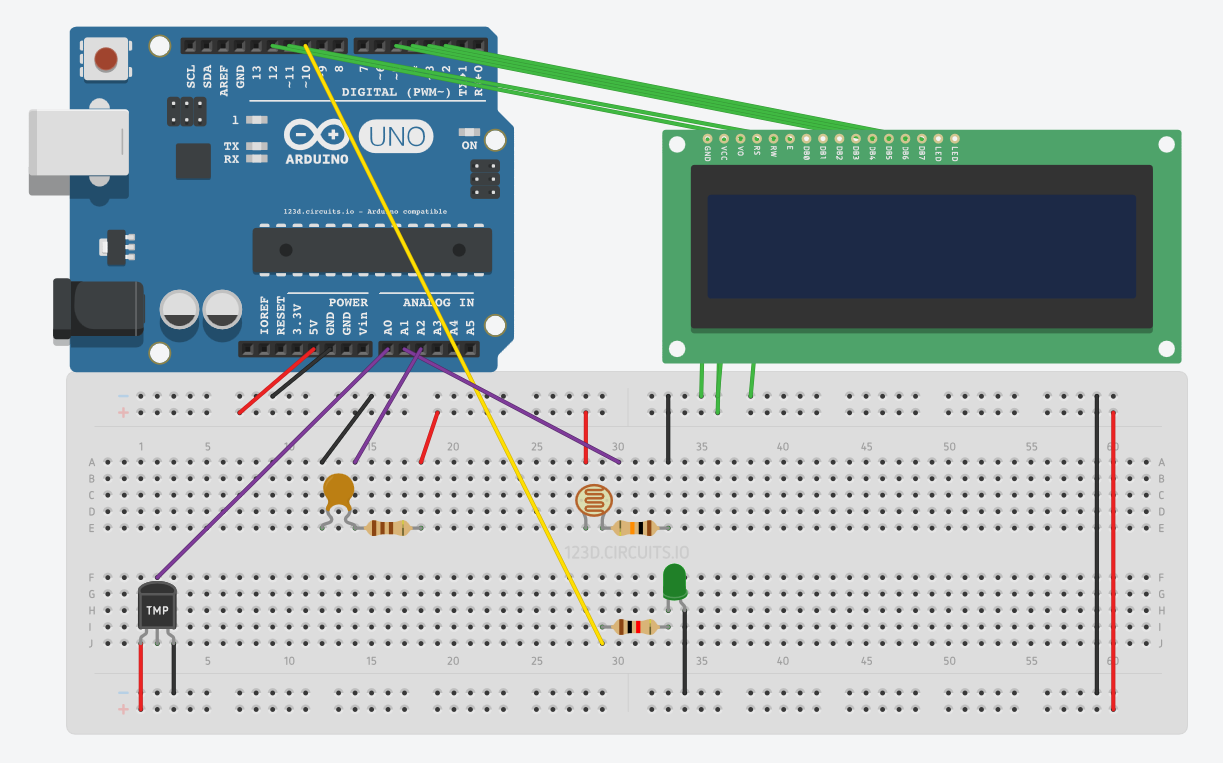
\includegraphics[width=1\linewidth]{images/squemaDibujo.PNG}
	\caption{Esquema global}
	\label{fig:squemadibujo}
\end{figure}


\begin{figure}[H]
	\centering
	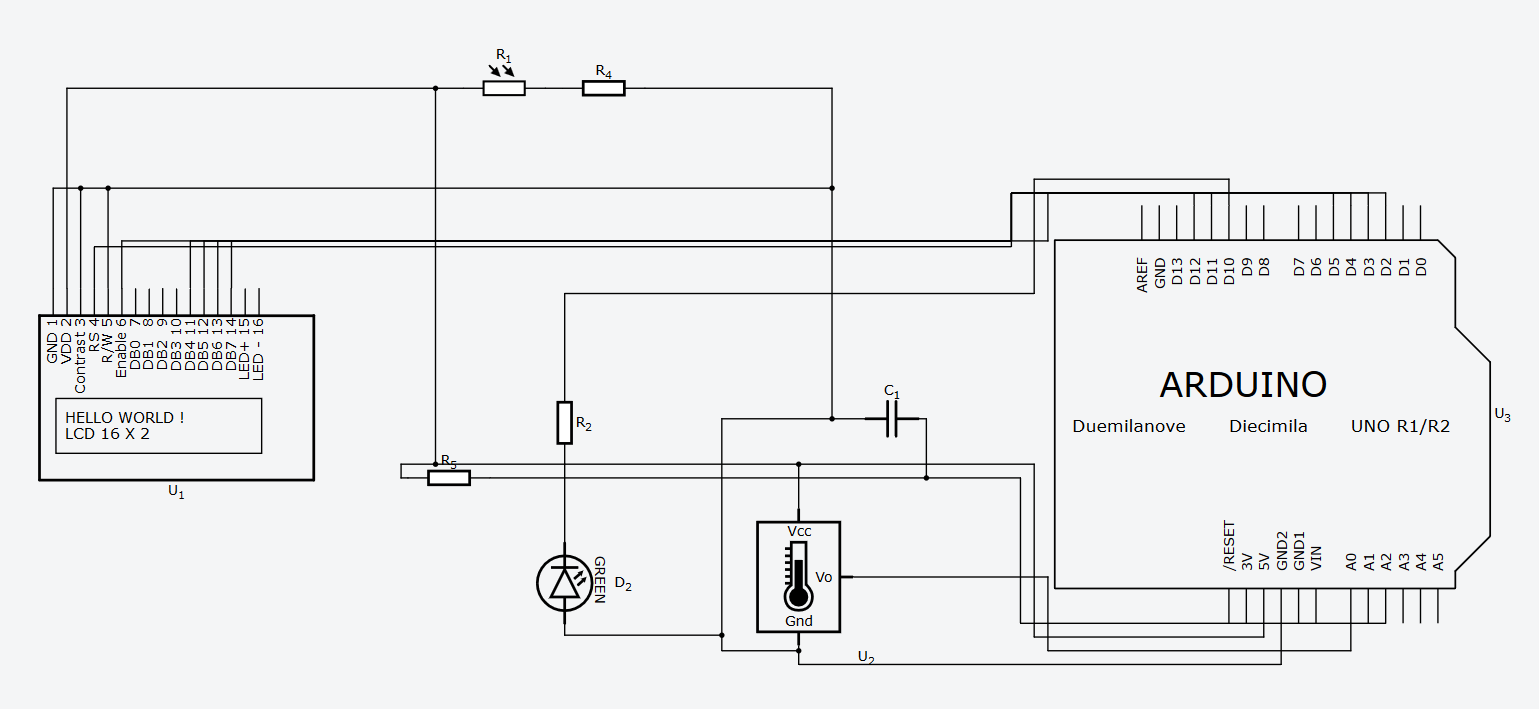
\includegraphics[width=0.6\linewidth]{images/squema.PNG}
	\caption{Esquema global}
	\label{fig:squema}
\end{figure}


\begin{figure}[H]
	\centering
	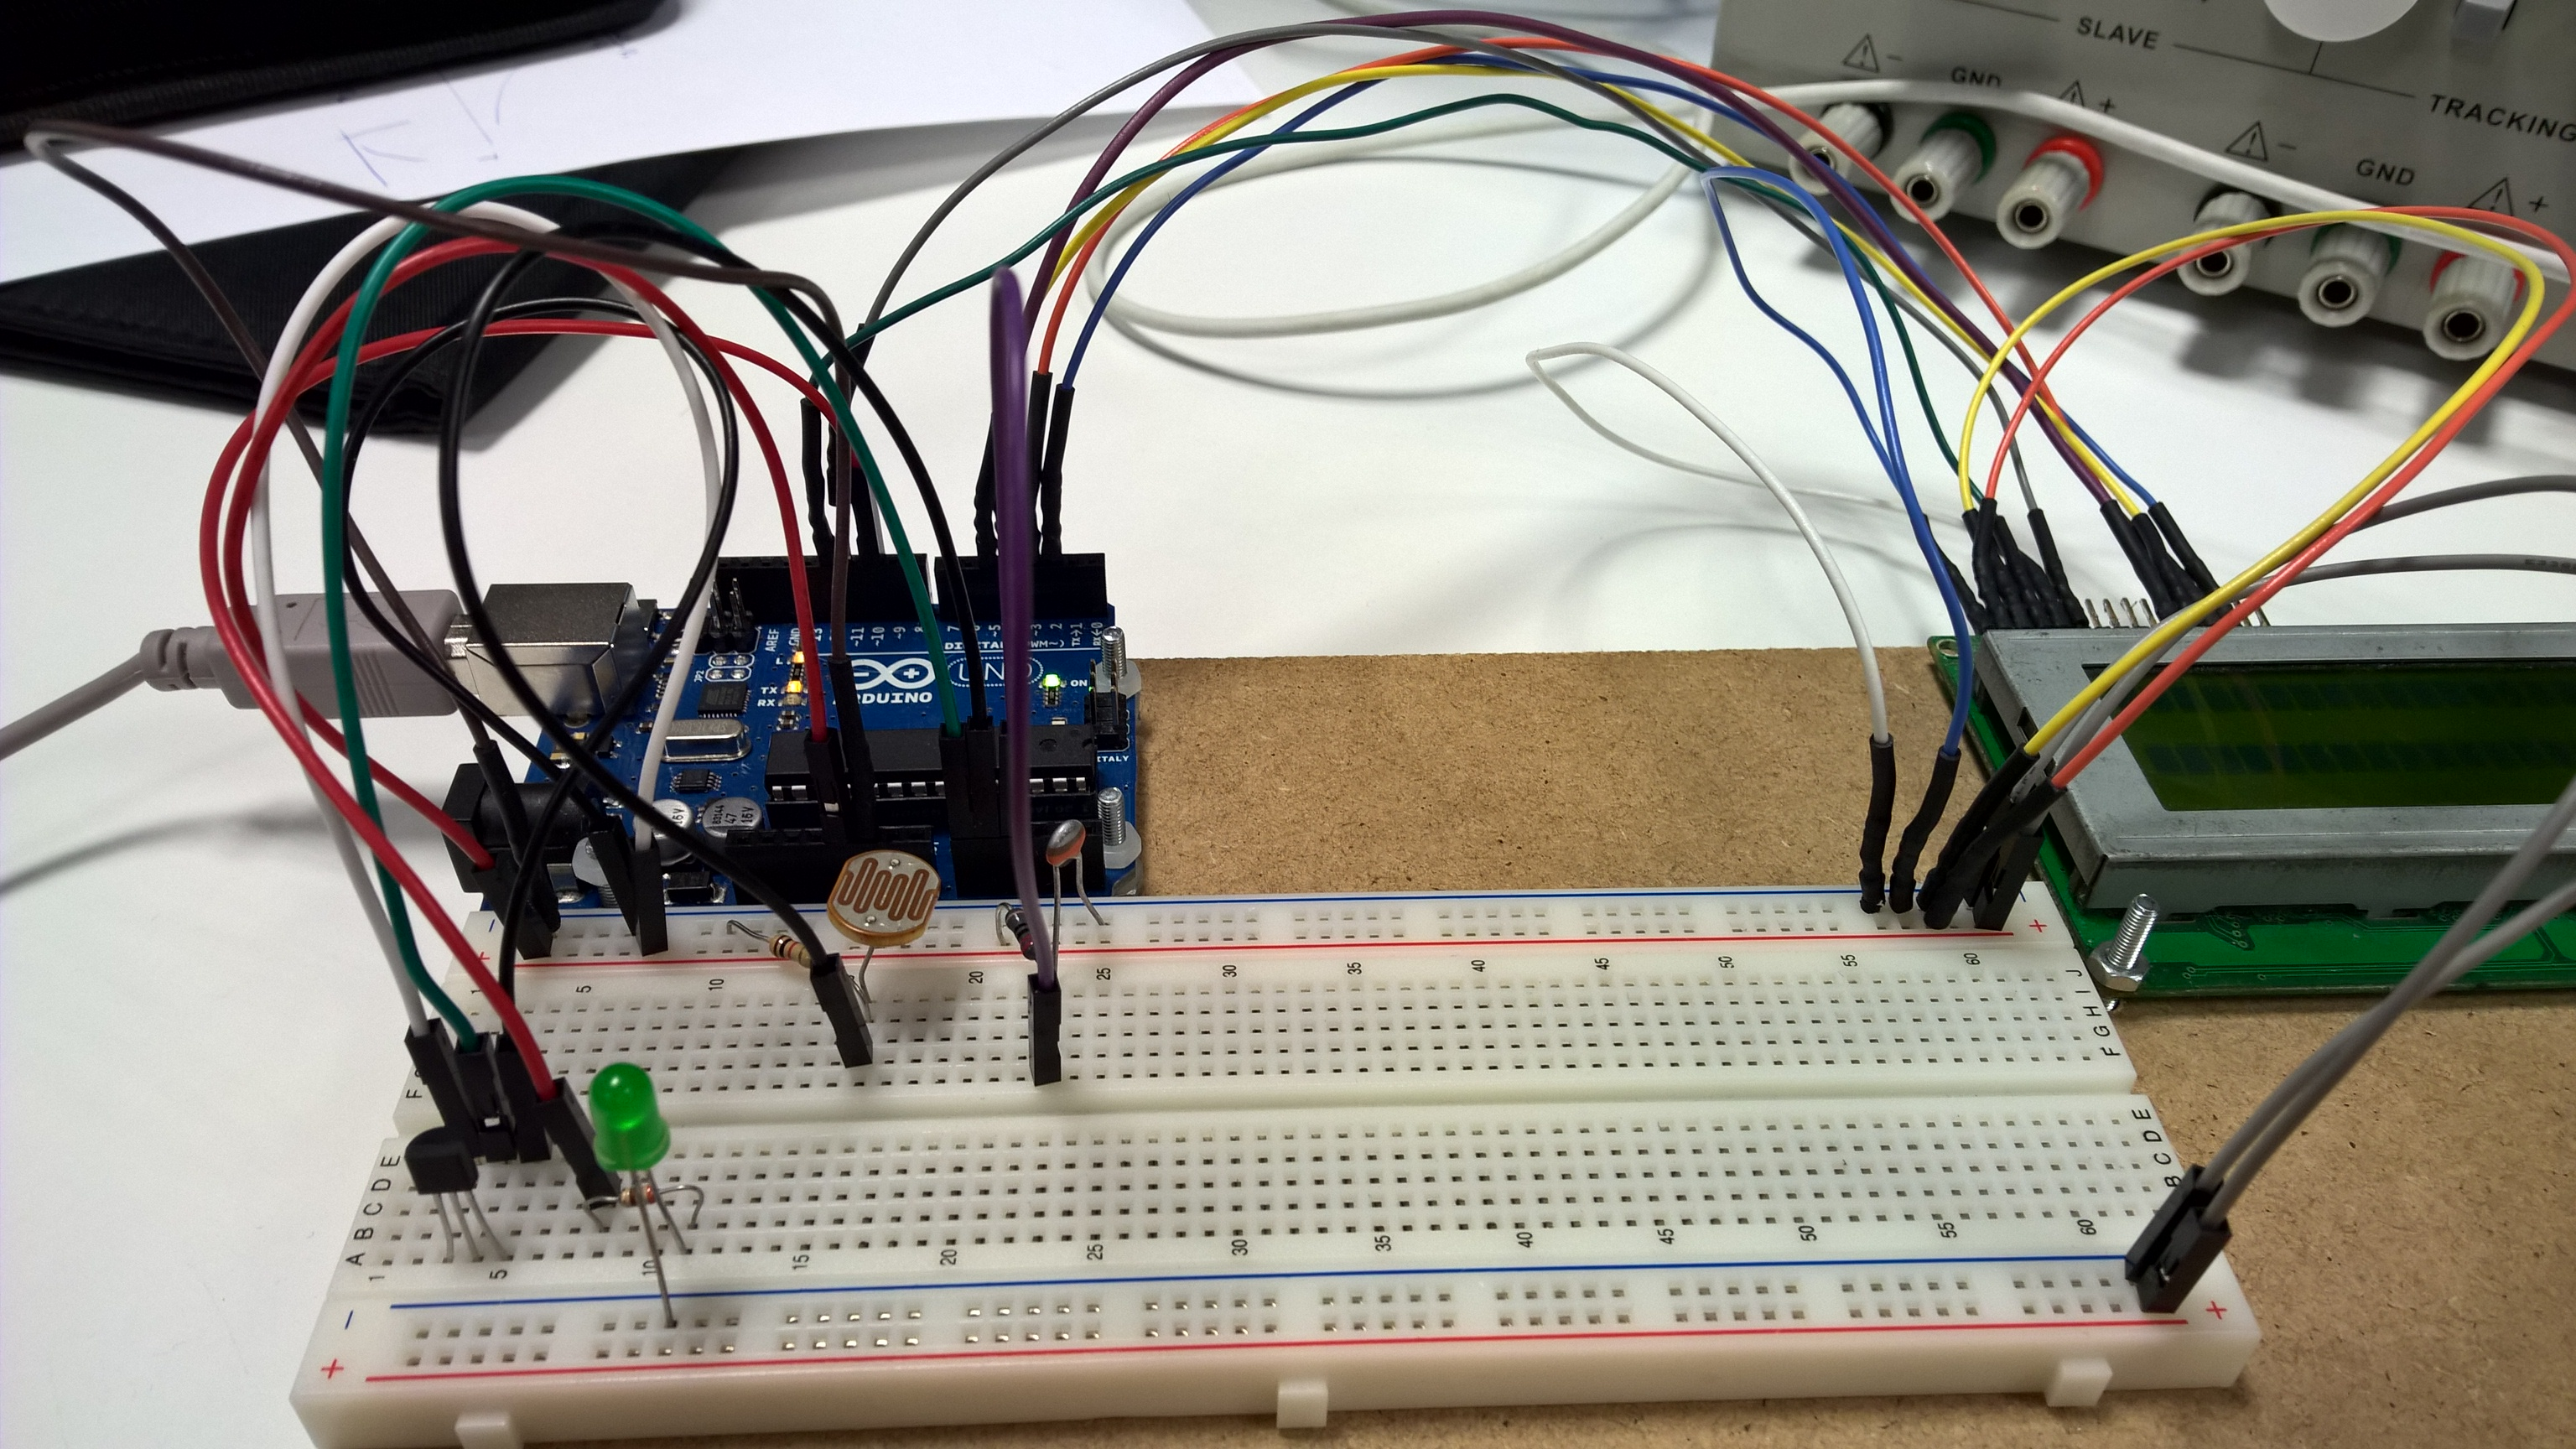
\includegraphics[width=1\linewidth]{images/arduinoUNO.jpg}
	\caption{Conexiones en Arduino UNO}
	\label{fig:uno}
\end{figure}

\begin{figure}[H]
	\centering
	\includegraphics[width=1\linewidth]{images/DUE2.jpg}
	\caption{Conexiones en Arduino DUE}
	\label{fig:due}
\end{figure}

\subsection{Led}
Un simple circuito de una resistencia y un Led en serie, donde el led se conecta a la señal GND de Arduino y por la resistencia al pin 10 (pwm).

En Arduino el código para poder controlar cuándo se enciende y apaga el led, y su intensidad por ser un pin pwm, primero en \textit{setup()} declaramos el pin 10 como de salida, y en el bucle de ejecución podemos llamar a la función \textit{digitalWrite(10, HIGH)} o con valor \textit{LOW}, para encender y apagar, o bien \textit{analogWrite(10, value)} con \textit{value} entre 0 y 255 para definir la intensidad del led.

\begin{figure}[H]
	\centering
	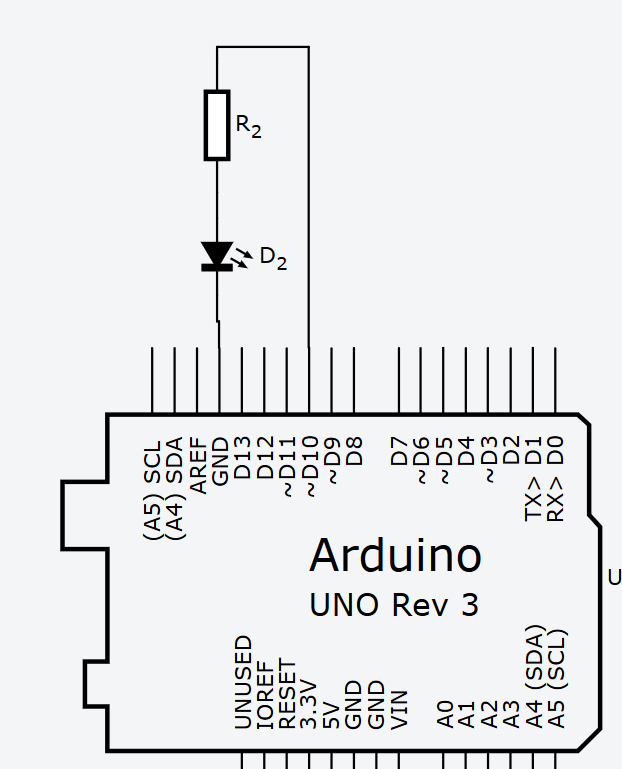
\includegraphics[width=0.4\linewidth]{images/led.PNG}
	\caption{Led}
	\label{fig:led}
\end{figure}

\subsection{Sensor de luz}

Siguiendo el esquema de la \autoref{fig:ldr} conectamos el sensor LDR a los pines de 5v, GND y analógico en el tramo de circuito que une el LDR y la resistencia, y en el código de Arduino realizamos un \textit{analogRead(A0)} de modo que leemos el valor del pin en cada iteración. Para pasarlo a valores positivos dentre del rango de 128 niveles de luz en el código realizamos al imprimir en la interfaz serie el valor: \textit{128 - analogRead(A0)/4}, como se puede leer en la sección final de código.

\begin{figure}[H]
	\centering
	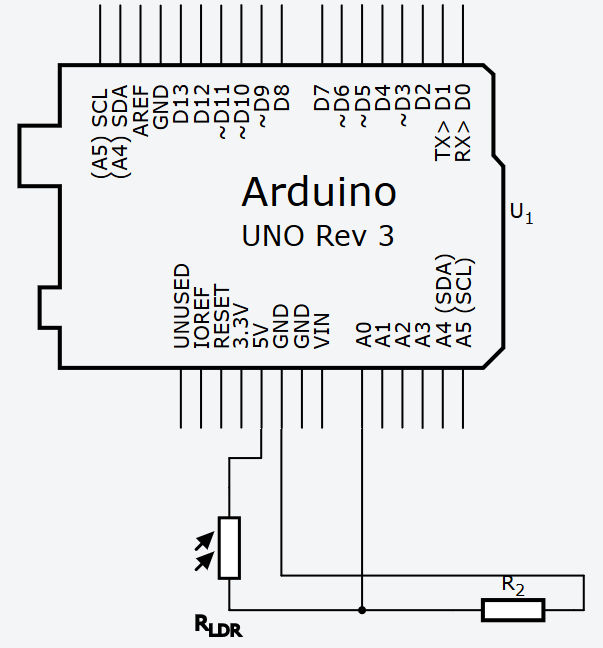
\includegraphics[width=0.4\linewidth]{images/ldr.PNG}
	\caption{LDR}
	\label{fig:ldr}
\end{figure}

\subsection{NTC}
El \textit{sensor de temperatura negativo} se conecta según el esquemático de la \autoref{fig:ntc} muy parecido al LDR. Tal y como indica la documentación de arduino \url{https://www.arduino.cc/en/Reference/AnalogRead} \textit{analogRead} devuelve un valor entre 0 y 1023 para voltajes entre 0 y 5 voltios, unos aprox. 4.9mV la unidad, y además debemos calibrar según los datos del fabricante, y la experimentación, la temperatura que devuelve.

En el código de la última sección se encuentran las transformaciones realizadas al valor leido, tanto en Arudino UNO como en el código Python de la Raspberry Pi.

\begin{figure}[H]
	\centering
	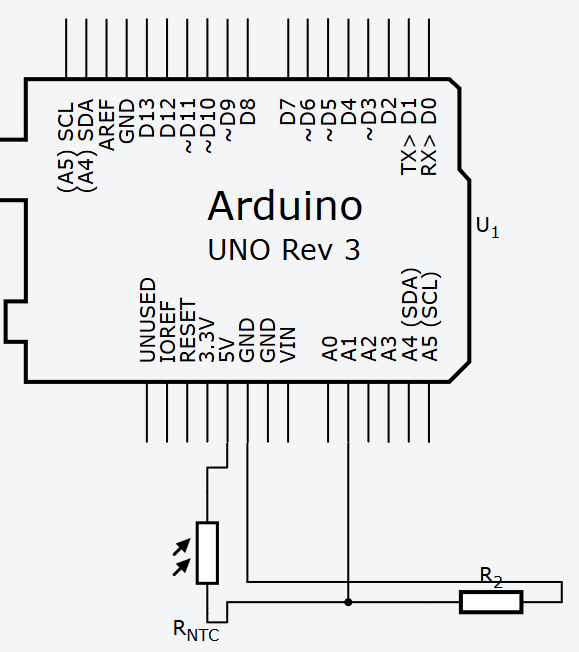
\includegraphics[width=0.4\linewidth]{images/ntc.PNG}
	\caption{NTC}
	\label{fig:ntc}
\end{figure}

\subsection{PTC}

Igual que el NTC, pero en vez de con lecturas de valores inversos al crecimiento de la temperatura, crece igual (de ahí que sean \textit{negativo} o \textit{positivo}). En el caso de la segunda parte de la práctica sólo usamos el NTC para medir la temperatura, pero en el código de Arduino UNO sí se encuentra el código que lee con \textit{analogRead} el valor del sensor, lo transforma, guiándonos por los datos del datasheet del fabricante y por datos experimentales para afinarlo.

\begin{figure}[H]
	\centering
	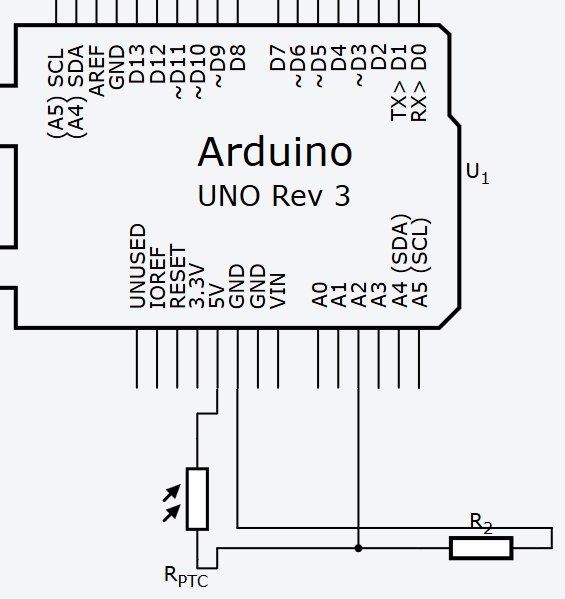
\includegraphics[width=0.4\linewidth]{images/ptc.PNG}
	\caption{PTC}
	\label{fig:ptc}
\end{figure}


\subsection{LCD}

El LCD tiene un buen soporte en Arduino, pues lo más \textit{complicado} es acertar a colocar los cables de los pines de Arduino y del LCD donde corresponden, pues luego tenemos la biblioteca \textit{LiquidCrystal.h} que con declarar el lcd por los pines con la orden \textit{LiquidCrystal lcd(12,11,5,4,3,2);}, inicializarlo con el tamaño de la pantalla \textit{lcd.begin(20,4)} ya tenemos preparada la pantalla para escribir con la orden \textit{lcd.pring("texto");}. Además, es muy útil la orden \textit{lcd.setCursor(0,0);} que permite volver al inicio de la pantalla para reescribir, en vez de anexar un texto detrás de otro.

Es de notar que la pantalla tiene 4 filas, pero escribe primero las impares y luego las pares, es decir, que de escribir un texto largo que ocupe toda la pantalla, habría que leer las líneas 1 y 3, y después seguir por la 2 y 4. En la segunda parte de la práctica, el servidor web habilita un cuadro de texto donde lo que se escriba se mostrará en el LCD, por ello primero se hace una reordenación del texto, de modo que cuando llegue como mensaje de nuestro protocolo propio al Arduino, se imprima correctamente por la pantalla.

\begin{figure}[H]
	\centering
	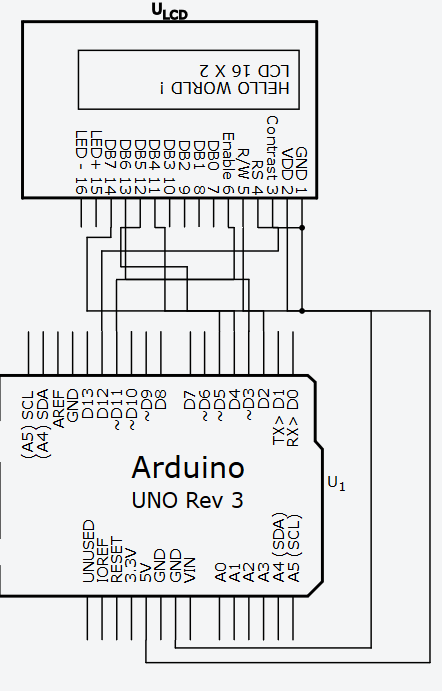
\includegraphics[width=0.4\linewidth]{images/lcd.PNG}
	\caption{LCD}
	\label{fig:lcd}
\end{figure}


\subsection{Generador señal tipo GPS}

Programamos el Arduino UNO para que genere una señal PN semejante a los códigos C/A de los GPS. Para ello nos basamos en el esquema de la \autoref{fig:gpsGen} y programamos el código en arduino, llegando a hacer operaciones a nivel de bits para conseguir la mayor eficiencia y la mayor velocidad posibles. En el código más abajo está comentado la impresión por pantalla del código, para comprobar que es correcto, y se emite por el pin 9, el cual conectamos al osciloscopio y conseguimos entre 45kHz y 66KHz.

\begin{figure}[h!]
	\centering
	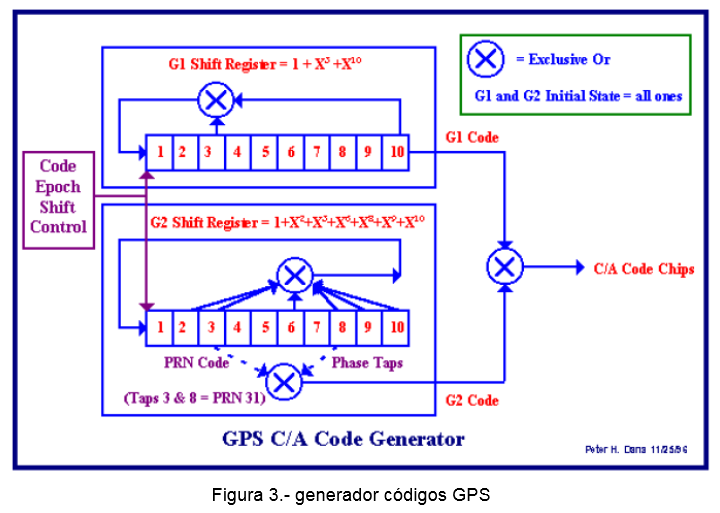
\includegraphics[width=0.6\linewidth]{images/gpsGen.PNG}
	\caption{Esquema generador códigos gps}
	\label{fig:gpsGen}
\end{figure}

Código Arduino UNO:

\lstinputlisting[language=C++,frame=single]{senialGPS.ino}

Muestras de osciloscopio por el pin 9:

\begin{figure}[h!]
	\centering
	\includegraphics[width=1\linewidth]{images/gps1.jpg}
	\caption{45.45kHz}
	\label{fig:gps1}
\end{figure}

\begin{figure}[h!]
	\centering
	\includegraphics[width=1\linewidth]{images/gps4.jpg}
	\caption{65.79kHz}
	\label{fig:gps4}
\end{figure}

Para la emisión por el módulo de radio frecuencia, como sólo acepta hasta un máximo de frecuencia, habría que reducirla con el uso de la orden \textit{delay()} en Arduino.


\section{Práctica 2. Montaje de un servidor web de monitorización. Descripción del software}

En la segunda parte de la práctica hemos puesto como objetivo desarrollar algo en el ámbito de internet de las cosas. Básicamente nuestro reto ha sido poner en internet (en nuestro caso usando HTTP y servicios Web) los distintos sensores y el monitor LCD utilizados en la práctica anterior.

Para ello nos hemos servido de un Arduino Due (ya que el voltaje de sus pines es compatible con la Raspberry Pi), de una Raspberry Pi y de un router Wifi que hace de punto de acceso entre la Raspberry Pi e internet.

\subsection{Montaje de red}

La Raspberry Pi, por su gran capacidad de cómputo, hace de centro de datos. Recibe información del Arduino Due a través de el puerto serie, y lo pone en internet a través de un puerto Ethernet. 

\begin{figure}[H]
\verbatiminput{net.txt}
\end{figure}

\begin{figure}[H]
	\centering
	\includegraphics[width=1\linewidth]{images/RASPI.jpg}
	\caption{Conexión Raspberry Pi}
	\label{fig:raspi}
\end{figure}

\subsection{Protocolo serie}

El protocolo serie es muy simple, y se basa en transmitir unas tramas con la siguiente información (en ese orden):

\begin{itemize}
	\item 1 byte nulo (valor 0) que inidica inicio de la trama. Se utiliza para sincronizar en caso de error.
	\item 4 bytes que codifican en ASCII hexadcimal el tamaño de la trama.
	\item 1 byte que codifica en ASCII el tipo del paquete.
		\subitem L: Valor de intensidad para el \textbf{L}ed.
		\subitem D: Texto para mostrar en el LCD \textbf{D}isplay.
		\subitem l: Información del sensor de \textbf{l}uz.
		\subitem t: Información del sensor de \textbf{t}emperatura.
	\item Varios bytes con el payload de la trama, en ASCII.
\end{itemize}


\textit{1 byte de sincronización +}
Paquete protocolo serie:
\begin{verbatim}
		+-------------------+-------+-------------........-----------------+
		|                   |  Tipo |                                      |
		| Longitud (4bytes) |  (1B) |         PAYLOAD (Longitud - 5 bytes) |
		|                   |       |                                      |
		+-------------------+-------+-------------........-----------------+
\end{verbatim}


\subsection{Código arduino}

Lo primero que hemos hecho ha sido reutilizar parte del código de la primera práctica. En un bucle continuo, leemos los sensores de temperatura y luz y con la información obtenida mandamos frames por el protocolo serie a la Raspberry Pi.

\hfill

Por otro lado, también nos encargamos de leer frames que puedan venir de la Rapsberry Pi. Si llega un frame de tipo 'L', le cambiamos el valor al \textit{analog output} del led, haciendo que ilumine más o menos. O por si llega un frame de tipo 'D', en cuyo caso limpiamos el display y ponemos el nuevo texto en la pantalla.

\subsection{Servicio web}
El servicio web tiene dos partes, un código escrito en python que corre en la Rapsberry PI y otro código escrito en javascript que se ejecuta en un teléfono móvil, o un pc.

\subsubsection{Parte servidor de python}
En esta parte, se espera a que un navegador web estándar haga una petición de tipo GET para obtener el documento index.html. Además, está a la espera de recibir peticiones GET al documento 'luz' o al documento 'tmp'.

\hfill

Cada vez que recibe una petición al documento luz, lee las tramas a través del puerto serie para obtener del Arduino la última lectura del sensor de luz. Después, contesta la petición con el valor del sensor. Lo mismo sucede si se recibe una petición al documento tmp, solo que se devuelve la temperatura.

\hfill

Por otro lado, el servidor de python también está a la espera de las peticiones PUT 'led' y 'display'. En este caso, en vez de devolver un valor leyendo por el puerto serie, lo que hace es escribir en el puerto serie una trama de tipo 'L' (si led) o de tipo 'D' (si display) para alterar el brillo del led o el texto del monitor LCD.

\subsubsection{Parte cliente de javascript}

En el explorador web, se ejecuta continuamente una petición de tipo GET 'luz' y GET 'tmp', para actualizar en tiempo real la oscuridad del fondo (dependiendo del nivel de luz), o el valor de un número dependiendo de la temperatura.

\hfill

También se pone una barra de desplazamiento para modificar el brillo del led, y una barra de texto para cambiar el mensaje del display. Cuando se mueve la barra de desplazamiento se ejecuta un PUT 'led', y cuando se cambia el texto en la barra se ejecuta un PUT 'display', que llegan al servidor web de python.




\begin{figure}[H]
	\centering
	\includegraphics[width=1\linewidth]{images/TEST1.jpg}
	\caption{Test 1: Slider intensidad Led. Temperatura ambiente. Luz ambiente. Mensaje en LCD.}
	\label{fig:test1}
\end{figure}

\begin{figure}[H]
	\centering
	\includegraphics[width=1\linewidth]{images/TEST2 luz.jpg}
	\caption{Test 2: Sombra en sensor de luz $\rightarrow$ fondo de la web más oscuro.}
	\label{fig:test2}
\end{figure}

\begin{figure}[H]
	\centering
	\includegraphics[width=1\linewidth]{images/TEST3 calor.jpg}
	\caption{Test 3: Temperatura de 120.66ºC por soldador.}
	\label{fig:test3}
\end{figure}

\section{Notas adicionales}

\subsection{Aproximación a la temperatura real}
Siguiendo las indicaciones de los fabricantes de los sensores de temperatura hemos llegado a lecturas que no pueden corresponderse con la realidad (porque aparecían disparates), así que hemos tenido que aproximar la temperatura con la experimentación.

%TODO: Exponer las fórmulas

\subsection{Lector de pulsaciones}
Al final del cuatrimestre pudimos experimentar con un sensor de pulsaciones del corazón. El sensor es muy sencillo de utilizar: la cara con circuitería se proteje con plástico o tela para que no toque la piel, pues las indicaciones avisan del impacto negativo de la grasa sobre el circuito, la otra cada se toca con la punta del dedo y se puede sujetar con un anillo de velcro; las conexiones son 3, tierra, voltaje, que soporta tanto 3,3v como 5v para poder usarlo en cualquier versión de Arduino, y el cable que se conecta a la entrada analógica para lectura.

Usando el osciloscopio pudimos averiguar que una vez está en contacto con el dedo, el sensor mantiene dos niveles de señal: aproximadamente 2v cuando no hay pulso, sólo contacto; 3.3v cuando se detecta un pulso.

De este modo, aunque no nos dio tiempo, la incorporación del sensor de pulsaciones a arduino sería hacer una lectura del sensor periódica y detectar los picos de tensión sobre los 3v, para dar margen de error al teórico 3.3v.

\section{Código}
\subsection{Código Arduino}

Dos ficheros, uno con el código de los sensores de la primera parte, usando el Arduino UNO, y el segundo el código de Arduino DUE con el protocolo de comunicación y lectura de sensores.


\textit{Código sensores Arduino UNO:}
\lstinputlisting[language=C++,frame=single]{codigoSensoresArduinoUNO.ino}

\textit{Código Arduino DUE:}
\lstinputlisting[language=C++,frame=single]{pser.ino}

\subsection{Código Raspberry Pi}

Dos ficheros, el servidor web escrito en Python, implementando el protocolo de comunicación con Arduino DUE, y el fichero \textit{index.html} de la página web que muestran la información de los sensores o entrada de datos para pantalla y led.

\textit{Código servidor Python:}
\lstinputlisting[language=Python,frame=single]{restserver.py}

\textit{Código página web:}
\lstinputlisting[language=html,frame=single]{index.html}

\end{document}
